\subsection{Original problem}

\subsubsection*{Optimal solution (one of them)}

The active power generated by the generator i, $P_{G_i}$: 

\begin{table}[!h]
    \centering
\begin{tabular}{|c|c|c|c|c|c|}
  \hline
  $P_{G_1}$ & $P_{G_2}$ & $P_{G_3}$ & $P_{G_4}$ & $P_{G_5}$ & $P_{G_6}$ \\
  \hline
  0.400 & 0.400 & 0.500 & 0.600 & 0.410 & 0.000 \\
  \hline
\end{tabular} \ .
\end{table}
\noindent
As expected we divide the generation of the active power ($2.31$ [pu]) among the cheapest generators, and as asked we match the demand exactly.\\

The reactive power generated/absorbed by the generator i, $Q_{G_i}$:
\begin{table}[!h]
    \centering
\begin{tabular}{|c|c|c|c|c|c|}
  \hline
  $Q_{G_1}$ & $Q_{G_2}$ & $Q_{G_3}$ & $Q_{G_4}$ & $Q_{G_5}$ & $Q_{G_6}$ \\
  \hline
  -0.042 & 0.000 & 0.042 & 0.000 & 0.000 & 0.000 \\
  \hline
\end{tabular} \ .
\end{table}

\noindent
The voltage amplitude of the node k, $U_k$:

\begin{table}[!h]
    \centering
\begin{tabular}{|c|c|c|c|}
  \hline
  $U_{1}$ & $U_{2}$ & $U_{3}$ & $U_{4}$ \\
  \hline
  0.902 & 0.904 & 0.901 & 0.900 \\
  \hline
\end{tabular} \ .
\end{table}

\noindent
The voltage phase angle of the node k, $\theta_k$:

\begin{table}[!h]
    \centering
\begin{tabular}{|c|c|c|c|}
  \hline
  $\theta_{1}$ & $\theta_{2}$ & $\theta_{3}$ & $\theta_{4}$ \\
  \hline
  0.005 & 0.017 & -0.007 & -0.014 \\
  \hline
\end{tabular} \ .
\end{table}

\noindent
The objective value, $z = 413.000$.\\

The two following figures represent the effective transmissions of the active and the reactive power respectively:

\begin{figure}[!h]
    \centering
    
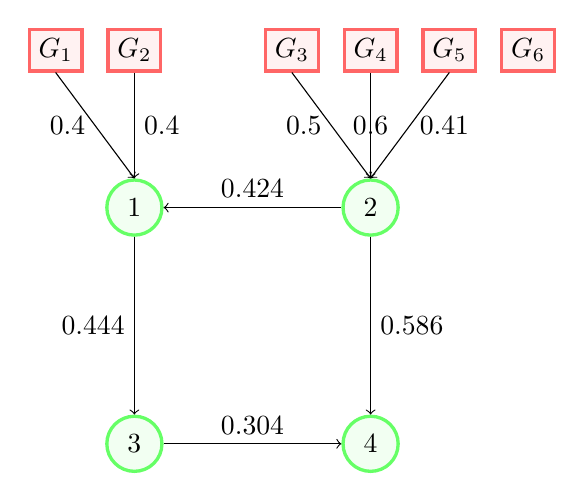
\begin{tikzpicture}[
roundnode/.style={circle, draw=green!60, fill=green!5, very thick, minimum size=7mm},
squarednode/.style={rectangle, draw=red!60, fill=red!5, very thick, minimum size=5mm},
]
%Nodes
\node[roundnode]    (node1)      at (0,0) {1};
\node[roundnode]    (node2)      at (3,0) {2};
\node[roundnode]    (node3)      at (0,-3) {3};
\node[roundnode]    (node4)      at (3,-3) {4};
\node[squarednode]  (gen1)       at (-1,2) {$G_1$};
\node[squarednode]  (gen2)       at (0,2) {$G_2$};
\node[squarednode]  (gen3)       at (2,2) {$G_3$};
\node[squarednode]  (gen4)       at (3,2) {$G_4$};
\node[squarednode]  (gen5)       at (4,2) {$G_5$};
\node[squarednode]  (gen6)       at (5,2) {$G_6$};
 
%Lines
\draw[<-] (node1.east) -- node[above] {$0.424$} (node2.west);
\draw[->] (node3.east) -- node[above] {$0.304$} (node4.west);
\draw[->] (node1.south) -- node[left] {$0.444$} (node3.north);
\draw[->] (node2.south) -- node[right] {$0.586$} (node4.north);
\draw[->] (gen1.south) -- node[left] {$0.4$} (node1.north);
\draw[->] (gen2.south) -- node[right] {$0.4$} (node1.north);
\draw[->] (gen3.south) -- node[left] {$0.5$} (node2.north);
\draw[->] (gen4.south) -- node {$0.6$} (node2.north);
\draw[->] (gen5.south) -- node[right] {$0.41$} (node2.north);
%\draw[->] (gen6.south) -- (node2.north);
%\draw[->] (node2.south) .. controls +(down:7mm) and +(right:7mm) .. (node3.east);
\end{tikzpicture}    
    
    \caption{Active Power Transmission [pu]}
    \label{fig:my_label}
\end{figure}

\begin{figure}[!h]
    \centering
    
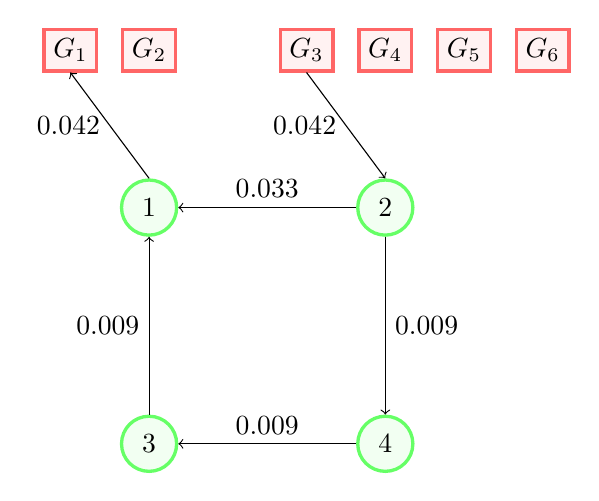
\begin{tikzpicture}[
roundnode/.style={circle, draw=green!60, fill=green!5, very thick, minimum size=7mm},
squarednode/.style={rectangle, draw=red!60, fill=red!5, very thick, minimum size=5mm},
]
%Nodes
\node[roundnode]    (node1)      at (0,0) {1};
\node[roundnode]    (node2)      at (3,0) {2};
\node[roundnode]    (node3)      at (0,-3) {3};
\node[roundnode]    (node4)      at (3,-3) {4};
\node[squarednode]  (gen1)       at (-1,2) {$G_1$};
\node[squarednode]  (gen2)       at (0,2) {$G_2$};
\node[squarednode]  (gen3)       at (2,2) {$G_3$};
\node[squarednode]  (gen4)       at (3,2) {$G_4$};
\node[squarednode]  (gen5)       at (4,2) {$G_5$};
\node[squarednode]  (gen6)       at (5,2) {$G_6$};
 
%Lines
\draw[<-] (node1.east) -- node[above] {$0.033$} (node2.west);
\draw[<-] (node3.east) -- node[above] {$0.009$} (node4.west);
\draw[<-] (node1.south) -- node[left] {$0.009$} (node3.north);
\draw[->] (node2.south) -- node[right] {$0.009$} (node4.north);
\draw[<-] (gen1.south) -- node[left] {$0.042$} (node1.north);
%\draw[->] (gen2.south) -- node[right] {$0.4$} (node1.north);
\draw[->] (gen3.south) -- node[left] {$0.042$} (node2.north);
%\draw[->] (gen4.south) -- node {$0.6$} (node2.north);
%\draw[->] (gen5.south) -- node[right] {$0.41$} (node2.north);
%\draw[->] (gen6.south) -- (node2.north);
%\draw[->] (node2.south) .. controls +(down:7mm) and +(right:7mm) .. (node3.east);
\end{tikzpicture}    
    
    \caption{Reactive Power Transmission [pu]}
    \label{fig:my_label}
\end{figure}


\newpage

\subsubsection*{Increase the capacity of one generator}

If it was possible to increase the capacity of one generator by $0.1$ pu, we would choose to increase the capacity of one of the cheapest generator that is $G_1$ or $G_3$. Without any additional computation, we would choose to increase the capacity of $G_3$ because we already know that there exist an optimal solution. Indeed, reducing the active power coming from the generator 5 by $0.1$ pu while increasing the active power coming from generator 3 by $0.1$ pu, doesn't change the other optimal values.\\
We can easily calculate the modification of the optimal value: \\
$z_{new} = z_{old} + 0.1 \cdot (100 - 300) = 413 - 20 = 393$ [SEK/h].

\subsection{Approximation of the OPF}
\subsubsection*{Optimal solution}
The active power generated by the generator i, $P_{G_i}$:

\begin{table}[!h]
    \centering
\begin{tabular}{|c|c|c|c|c|c|}
  \hline
  $P_{G_1}$ & $P_{G_2}$ & $P_{G_3}$ & $P_{G_4}$ & $P_{G_5}$ & $P_{G_6}$ \\
  \hline
  0.400 & 0.400 & 0.500 & 0.600 & 0.410 & 0.000 \\
  \hline
\end{tabular} \ ,
\end{table}
\noindent
which is exactly the same as in the non-linear model.\\

The voltage phase angle of the node $k$, $\theta_k$:

\begin{table}[!h]
    \centering
\begin{tabular}{|c|c|c|c|}
  \hline
  $\theta_{1}$ & $\theta_{2}$ & $\theta_{3}$ & $\theta_{4}$ \\
  \hline
  -0.010 & 0.000 & -0.020 & -0.0026 \\
  \hline
\end{tabular} \ ,
\end{table}
\noindent
the difference of voltage phase angle between the node $k$ and the node $m$ denoted $\theta_{k,m} = \theta_k - \theta_m$ are small between all the nodes (thus our approximations make sense).\\

The objective value, $z = 413.000$.
\subsection{Comparison}

\subsubsection*{Dual variables associated with the power flow balance constraint at each node}

The dual variables are given in the column called \textit{MARGINAL} in the output of the GAMS code.\\

If we look at the problem without constraint on the active power transmission in the links, then for both the non-linear and the approximate model the dual variable associated with the active power flow-balance constraint is equal to $300.0$ [SEK/pu/h] for each node. We can interpret those dual variables as the price to generate more active power on that node. If we increase the demand of active power of any node (until a certain limit) then the cost would raise by $300.0$ [SEK/pu/h] because the active power would be generated by $G_3$.\\

If we look at the problem with constraint on the active power transmission in the links, then in some case the dual variables have different values depending on the node. The reason is that due to the new constraints, if we increase the demand then depending on the node the active power could be generated on different generators (with different costs).

\subsubsection*{Imposing bounds on the active power transmission in the links}

We want to observe the sensitivity (feasibility and modification of optimal value) of our non-linear and approximate problem to the establishment of bounds on the active power transmission in the links. If we impose bounds higher than the optimal active power transmission in the links, then there is no difference.\\
The feasibility of the problem also depends if we are able to give more power than demanded to one node or not. Here we assumed that the power flowing into the node minus the power flowing out of the node must be equal to the demand and not greater or equal!\\

First we look at the \textbf{approximate model}. We cannot reduce the active power transmission for the links $\{2,1\}$ and $\{2,4\}$ since the optimal power transmissions ($0.424$ and $0.586$ respectively) are already the minimum for those links. Nevertheless we can reduce the two other links $\{2,1\}$ and $\{2,4\}$ until no power is generated in the two first generators. With those bounds the new optimal value is $584$ SEK.

\begin{figure}[!h]
    \centering
    
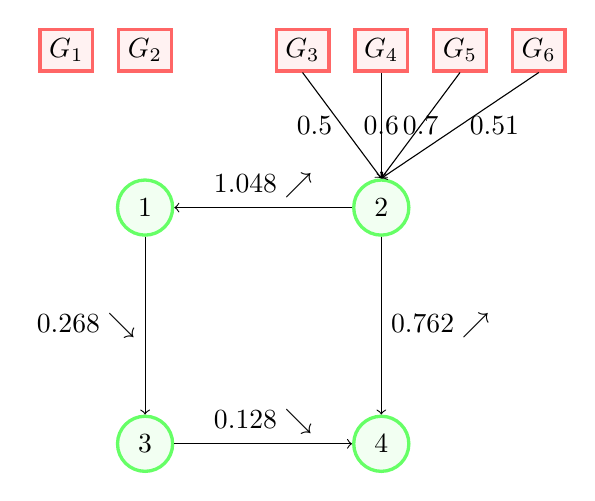
\begin{tikzpicture}[
roundnode/.style={circle, draw=green!60, fill=green!5, very thick, minimum size=7mm},
squarednode/.style={rectangle, draw=red!60, fill=red!5, very thick, minimum size=5mm},
]
%Nodes
\node[roundnode]    (node1)      at (0,0) {1};
\node[roundnode]    (node2)      at (3,0) {2};
\node[roundnode]    (node3)      at (0,-3) {3};
\node[roundnode]    (node4)      at (3,-3) {4};
\node[squarednode]  (gen1)       at (-1,2) {$G_1$};
\node[squarednode]  (gen2)       at (0,2) {$G_2$};
\node[squarednode]  (gen3)       at (2,2) {$G_3$};
\node[squarednode]  (gen4)       at (3,2) {$G_4$};
\node[squarednode]  (gen5)       at (4,2) {$G_5$};
\node[squarednode]  (gen6)       at (5,2) {$G_6$};
 
%Lines
\draw[<-] (node1.east) -- node[above] {$1.048 \nearrow$} (node2.west);
\draw[->] (node3.east) -- node[above] {$0.128 \searrow$} (node4.west);
\draw[->] (node1.south) -- node[left] {$0.268 \searrow$} (node3.north);
\draw[->] (node2.south) -- node[right] {$0.762 \nearrow$} (node4.north);
%\draw[->] (gen1.south) -- node[left] {$0.4$} (node1.north);
%\draw[->] (gen2.south) -- node[right] {$0.4$} (node1.north);
\draw[->] (gen3.south) -- node[left] {$0.5$} (node2.north);
\draw[->] (gen4.south) -- node {$0.6$} (node2.north);
\draw[->] (gen5.south) -- node {$0.7$} (node2.north);
\draw[->] (gen6.south) -- node[right] {$0.51$} (node2.north);
%\draw[->] (gen6.south) -- (node2.north);
%\draw[->] (node2.south) .. controls +(down:7mm) and +(right:7mm) .. (node3.east);
\end{tikzpicture}    
    
    \caption{Active Power Transmission with bounds on the active power transmission in the links [pu]}
    \label{fig:my_label}
\end{figure}


\newpage

We can not reduce the transmission in the link $\{2,1\}$. Indeed, if we want to reduce the transmission in that link then we can not meet the demand of the first node for two reasons:
\begin{enumerate}
    \item $G_1$ and  $G_2$ can not generate more active power, they already reached their maximum capacity.
    \item If we reduce the transmission of active power in the link $\{2,1\}$, we have to reduce the one in the link $\{1,3\}$ and in the link $\{3,4\}$ while increasing the one in the link $\{2,4\}$. Since the transmission of active power only depends on the voltage phase angle difference ($\theta_{k,m} = \theta_k - \theta_m$) this means that $\searrow \theta_{2,1}$, $\searrow \theta_{1,3}$, $\searrow \theta_{3,4}$ while $\nearrow \theta_{2,4}$, but this is impossible because $\theta_{2,1} + \theta_{1,3}+\theta_{3,4} = \theta_{2,4}$. 
\end{enumerate}

And we can not reduce the transmission in the link $\{2,4\}$ for a similar reason ($\nearrow  \theta_{2,1}$, $\nearrow \theta_{1,3}$, $\nearrow \theta_{3,4}$ while $\searrow \theta_{2,4}$).\\

Finally we look at the \textbf{non-linear model} and we observe that the bounds on the active power transmission in the links are almost the same. The only difference is that we can reduce a little the transmission in the link $\{2,1\}$ and in the link $\{2,4\}$ because the transmission depends on the voltage phase angle differences \underline{and} on the voltage amplitudes which are not constant anymore!

\subsubsection*{Bounds on the optimal value}

The linear approximation problem relaxed the constraint of the reactive power. So a feasible point in the approximate problem may be unfeasible in the original problem. In fact, the point calculated by the SNOPT solver in GAMS is not feasible in the original problem. However the approximation gives a fairly accurate estimation of the magnitude of the optimal value of the original problem.\\ 

If the approximation removes only some or all of the constraints then this approximation will give a minimum bound of the optimal value of the original problem. This is because that all the values the original problem can archive is achievable by the approximation problem but not verse vice. But the approximation done in this problem involve further constraints of the feasible domains as the voltage is limited to be equal to 1 and the voltage phase angles are limited to be close to each other. This might give a greater optimal value than the original problem. So this linearization approximation cannot give a bound for the optimal value of the original problem.\\ 

However from the resulting feasible points calculated with the original problem, it can be observed that the approximation is reasonable and that the optimal values conincide. \\

\textbf{Other method:} if we want a lower bound we could simply calculate the cost of distributing the demand of active power on the cheapest generators, without worrying about the feasability of the problem, the lower bound would be $413.0$ SEK. Then if we find values for the variables $P_{G_i}, Q_{G_i} U_k, \theta_k$ respecting the constraints such as the objective value is equal to $413.0$ SEK then we know that those values are optimal. But that bound do not give any hint on the feasibility of our problem.